% !TEX TS-program = XeLaTeX
% Commands for running this example:
% 	 xelatex Vahid-Proposal
% 	 xelatex Vahid-Proposal
% End of Commands

%%%  نمونه یک پروپوزال کارشناسی ارشد

% توجه داشته باشید برای دیدن خروجی کامل شامل نمایه و فهرست مطالب در ویرایشگر Texmaker، ابتدا دو بار 
% کلید F1 و بعد کلید F12 و دوباره کلید F1 و در آخر کلید F7 را فشار دهید.
%توضیحات مربوط به هر بسته یا دستور را می‌توانید در خط بالای آن ببینید.

\documentclass[12pt,a4paper,oneside]{book}
\usepackage[top=40mm, bottom=40mm, left=25mm, right=35mm]{geometry}
\usepackage{fancyhdr}
%در ورژن جدید زی‌پرشین برای تایپ متن‌های ریاضی، این سه بسته، حتماً باید فراخوانی شود
\usepackage{amsthm,amssymb}
\usepackage[table]{xcolor}% http://ctan.org/pkg/xcolor
\usepackage{float}
%دستوری برای وارد کردن واژه‌نامه انگلیسی به فارسی
\newcommand\persiangloss[2]{#1\dotfill\lr{#2}\\}
%بسته‌ای برای تنطیم حاشیه‌های بالا، پایین، چپ و راست صفحه
%\usepackage[top=50mm, bottom=50mm, left=50mm, right=50mm]{geometry}
%بسته‌ای برای نمایش تصاویر قرار داده شده در متن
\usepackage{graphicx}
\usepackage{standalone}
\usepackage{tikz}
\usetikzlibrary{shapes,arrows}
\usepackage[ruled]{algorithm}
\usepackage{algorithmic}
\usepackage{pgfplots}
\pgfplotsset{compat=newest}
\usepackage{standalone}
\usepackage{caption}
\usepackage{subcaption}
% بسته‌ و دستوراتی برای ایجاد لینک‌های رنگی با امکان جهش
\usepackage[pagebackref=false,colorlinks,linkcolor=blue,citecolor=blue]{hyperref}
% چنانچه قصد پرینت گرفتن نوشته خود را دارید، خط بالا را غیرفعال و  از دستور زیر استفاده کنید چون در صورت استفاده از دستور زیر‌‌، 
% لینک‌ها به رنگ سیاه ظاهر خواهند شد و برای پرینت گرفتن، مناسب‌تر خواهد بود
%\usepackage[pagebackref=false]{hyperref}
%بسته‌ای برای ظاهر شدن «مراجع» و «نمایه» در فهرست مطالب
\usepackage{tocbibind}
\usepackage{notoccite}
%دستورات زیر جهت هماهنگ شده با قالب دانشگاه علم و صنعت اضافه شده است.
\usepackage[fleqn]{amsmath}
\usepackage{titlesec}
%%%%%%%%%%%%%%
%فراخوانی بسته زی‌پرشین و دستورات مربوط به نوع فونت‌ها
\usepackage{fontspec}
\usepackage{xepersian}
\settextfont[Path = ./fonts/,Scale=1]{XB Niloofar}
% از revision 118 زی‌پرشین به بعد، وارد کردن دستور زیر لازم نیست. توجه داشته باشید که در صورت  غیرفعال کردن این دستور،
% از فونت پیش‌فرض لاتک برای کلمات انگلیسی استفاده خواهد شد.
%\setlatintextfont[ExternalLocation,BoldFont={lmroman10-bold},BoldItalicFont={lmroman10-bolditalic},ItalicFont={lmroman10-italic}]{lmroman10-regular}
% چنانچه می‌خواهید که اعداد در فرمول‌ها، فارسی باشد، دستور زیر را فعال کنید
%\setdigitfont{XB Zar}
%%%%%%%%%%%%%%%%%%%%%%%%%%%%%%%%%%%%%%%%%%%%%%%%%%%
% تعریف قلم‌های فارسی و انگلیسی برای استفاده در بعضی از قسمت‌های متن
\defpersianfont\titr[Path = ./fonts/,Scale=1]{XB Titre}
\defpersianfont\nastaliq[Path = ./fonts/,Scale=1.5]{XB Niloofar}
%\defpersianfont\traffic[Scale=1]{B Traffic}
%\defpersianfont\yekan[Scale=1]{B Yekan}
%اگر فونت‌های بالا را ندارید، دو خط بالا را غیر فعال و دو خط زیر را فعال کنید
\defpersianfont\traffic[Path = ./fonts/,Scale=1]{XB Roya}
\defpersianfont\yekan[Path = ./fonts/,Scale=1]{XB Kayhan}
%%%%%%%%%%%%%%%%
%%%%%%%%%%%%%%%%

\newcommand{\norm}[1]{\left\lVert#1\right\rVert}


\theoremstyle{definition}
\newtheorem{definition}{تعریف}
\newtheorem{theorem}{قضیه}
\newtheorem{lemma}{لم}
\newtheorem{proposition}{گزاره}
\newtheorem{corollary}{نتیجه}
\newtheorem{remark}{ملاحظه}
\theoremstyle{definition}
\newtheorem{example}{مثال}
%%%%%%%%%%%%%%%%%%


\pagestyle{fancy}
\fancyhf{}

\fancyhead[LE,LO]{\nouppercase{\leftmark}}
\fancyfoot[C]{\thepage}

\renewcommand\headrulewidth{1.5pt}
\makeatletter
\def\headrule{{\if@fancyplain\let\headrulewidth\plainheadrulewidth\fi
\hrule\@height\headrulewidth\@width\headwidth
\vskip 2pt% 2pt between lines
\hrule\@height.5pt\@width\headwidth% lower line with .5pt line width
\vskip-\headrulewidth
\vskip-1.5pt}}
\makeatother

%%%%%%%%%%%%%%%%%%
\SepMark{-}
%%%%%%%%%
 \titleformat{\chapter}[display]
{\vspace{-3cm}\vfill\filcenter}
{{%
   \vspace{-3cm}\filcenter\fontsize{48pt}{48pt}\selectfont{\chaptername}
   \fontsize{48pt}{48pt}\selectfont\thechapter%
 }%
}
{50pt}
{\fontsize{30pt}{30pt}\selectfont%
}[\vfill\clearpage]
\titlespacing*{\chapter}{0pt}{0pt}{0pt}
%%%%%%%%%%%%%%%%
%%%%%%%%%%%%%% HB %%%%%%%%%%%%%%%%
\usepackage{bm}
\usepackage[font=scriptsize,labelfont=bf]{caption}
\usepackage{perpage}
 \MakePerPage{footnote}
%%%%%%%%%%%%%% HB %%%%%%%%%%%%%%%%
\def\C{ \mathbb{C}}
\def\R{\mathbb{R}}
\def\Z{ \mathbb{Z}}
\def\N{ \mathbb{N}}

%%%%%%%%%%%%%%%%

\begin{document}

% دستوری جهت ظاهر نشدن شماره صفحه و سربرگ، در صورت وجود (فقط در صفحه جاری)
\thispagestyle{empty}
\vspace*{-28mm}
% نحوه درج کردن لوگوی دانشگاه
\centerline{
\includegraphics[scale=0.1]{./Images/general/logo.png}}
\begin{center}
%دستوری برای کم کردن فاصله بین لوگو و خط پایین آن
\vspace{-1mm}
\textbf{دانشکده فنی و مهندسی}
%دستوری برای تعیین فاصله بین دو خط
\\[3cm]
\begin{Huge}
\textbf{
بررسی و کاهش کوپلینگ متقابل در آنتن های میکرواستریپ
}
\end{Huge}
\\[1.5cm]
\Large
گزارش پایانی پروژه‌ی کارشناسی
\\[0.25cm]
در رشته‌ی مهندسی برق گرایش مخابرات
\\[3cm]
دانشجو:
\\[0.25cm]
\textbf{
محمد حسن بهشتی    
\\[1cm]
استاد راهنما:
\\[0.25cm]
دکتر حمیدرضا حسنی
\\[1cm]
شهریور ماه ۱۴۰۴
}
\end{center}
\newpage
\thispagestyle{empty}
\centerline{\includegraphics[scale=0.75]{./Images/general/besmallah.jpg}}

\newpage
\thispagestyle{empty}
\centerline{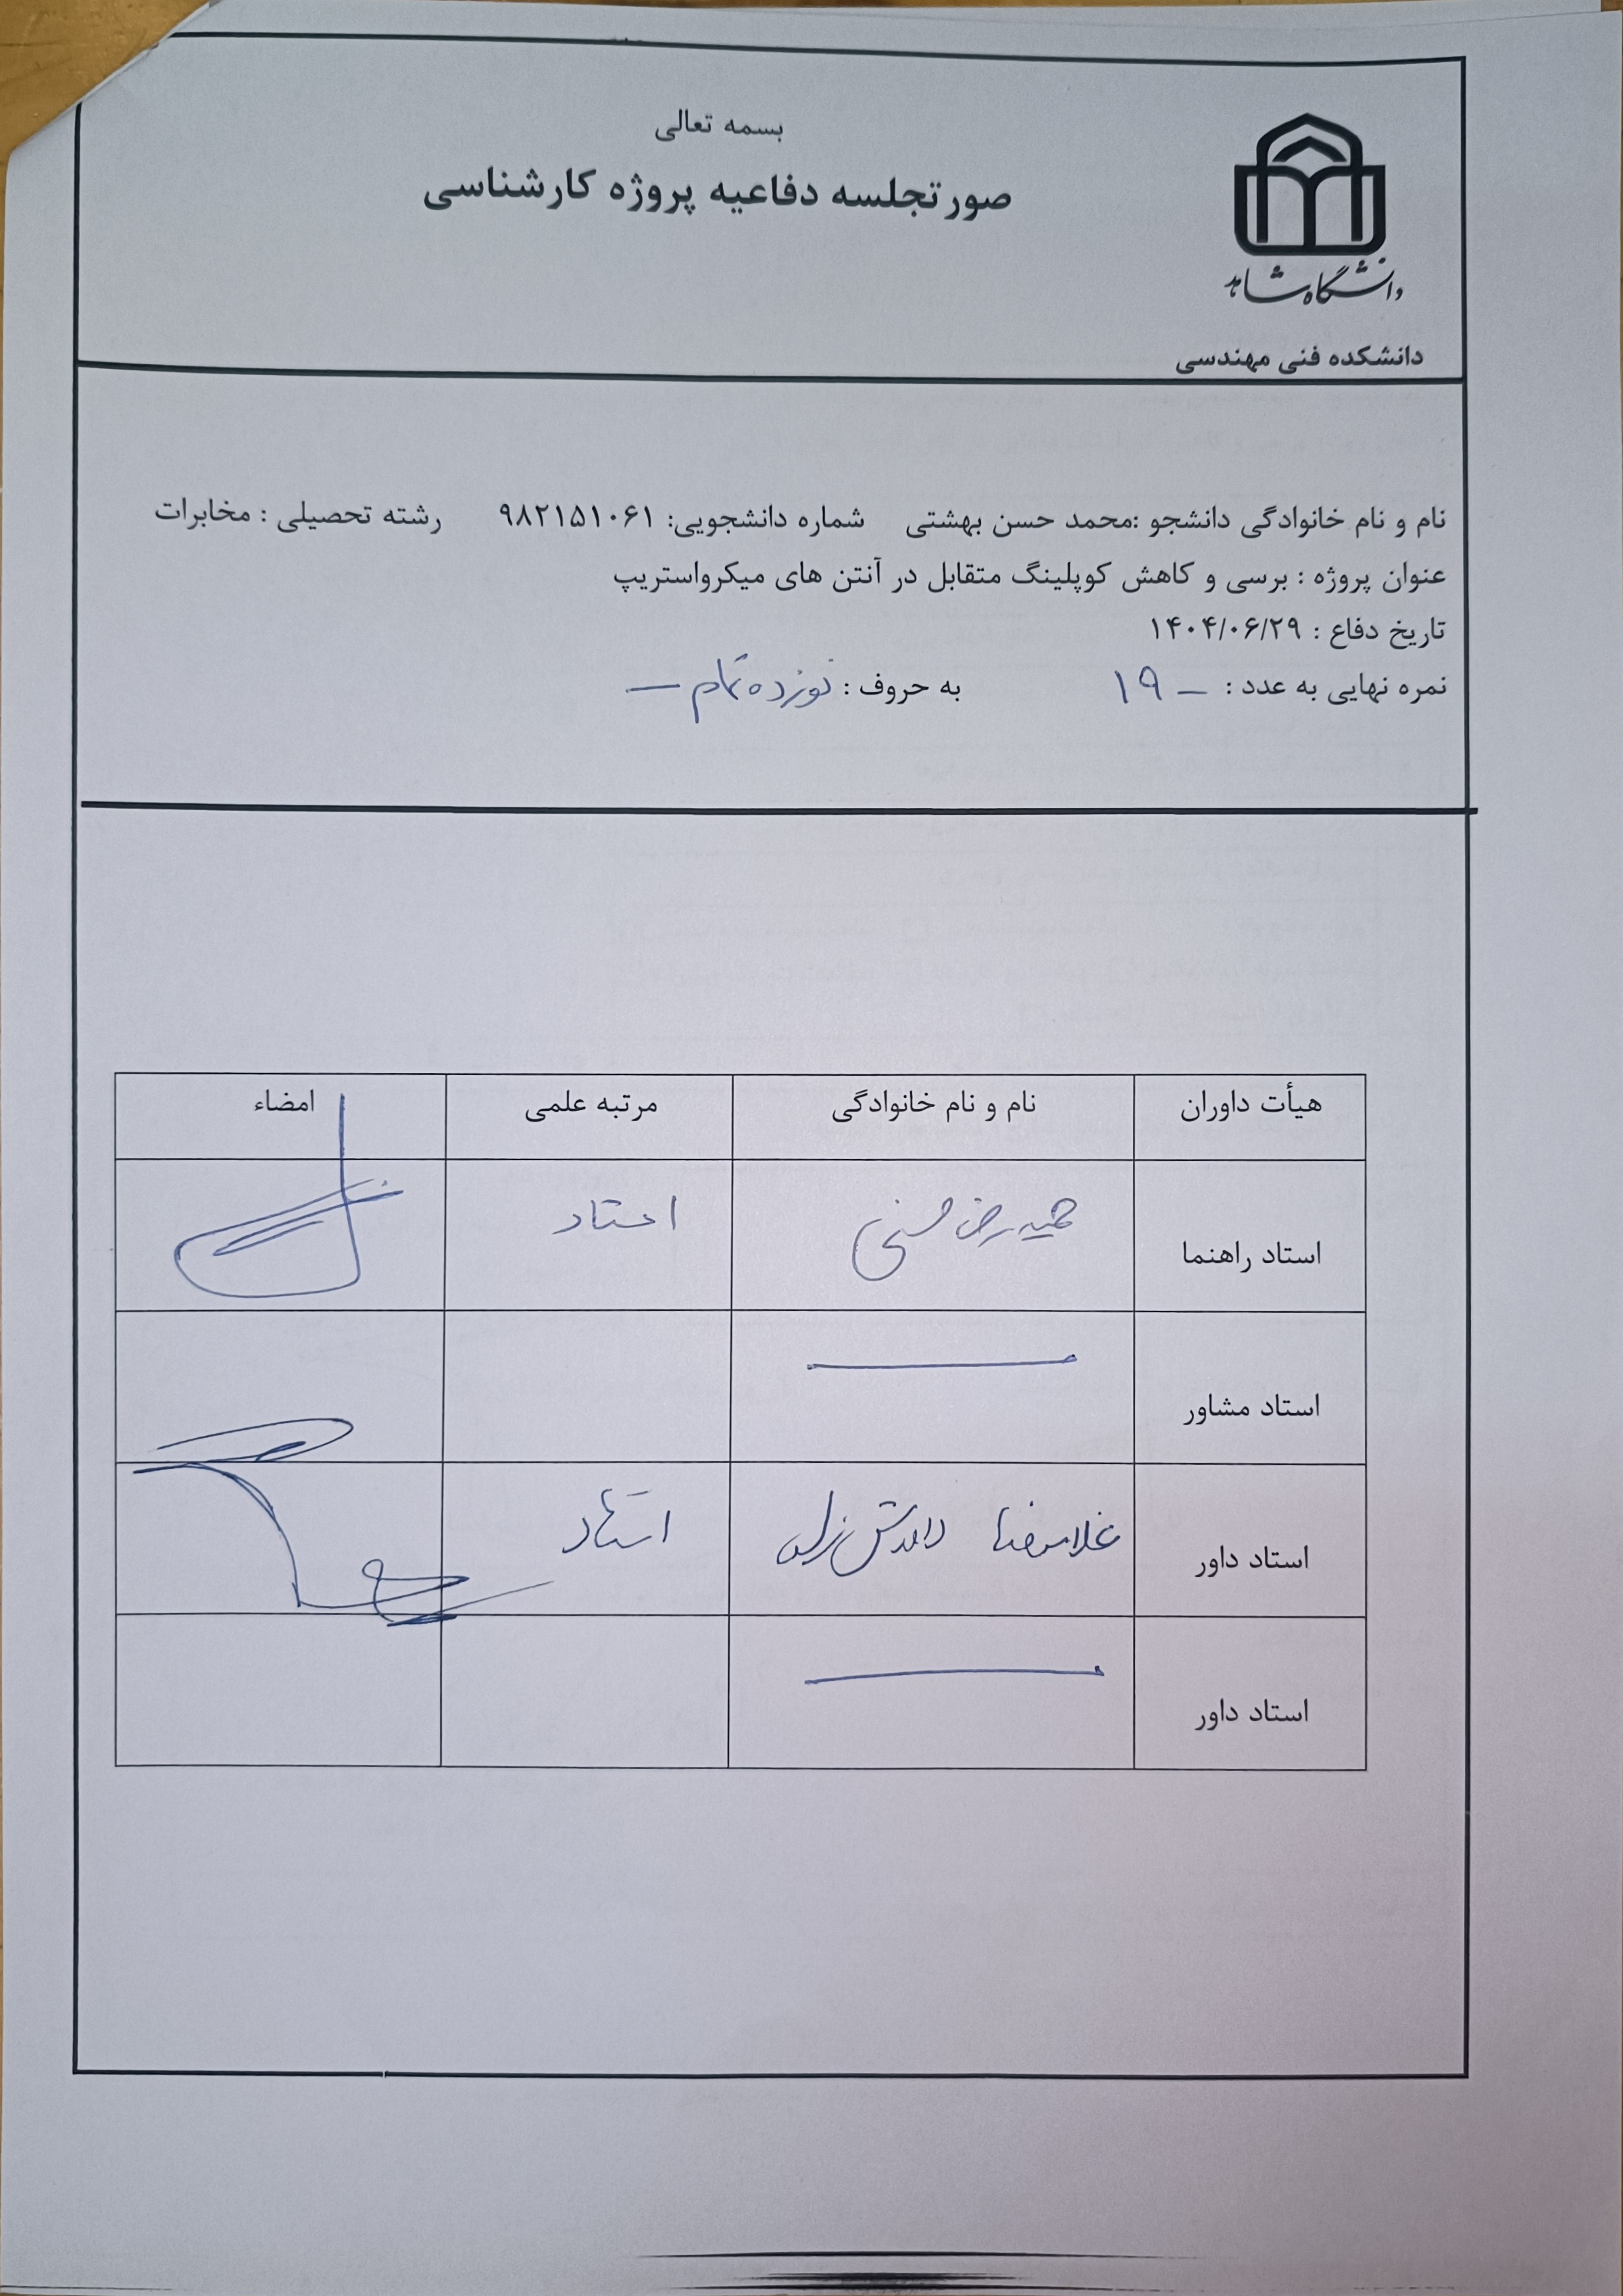
\includegraphics[scale=0.2]{./Images/general/soorat.jpg}}
\pagenumbering{harfi}
%دستوری برای ظاهر شدن فهرست مطالب
\tableofcontents
\newpage
\listoffigures

\baselineskip=1cm
\newpage 
\chapter*{چکیده}
\thispagestyle{empty}
\section*{چکیده}

آنتن‌های میکرواستریپ به دلیل سادگی ساخت و ابعاد کوچک کاربرد وسیعی در سامانه‌های مخابراتی دارند. با این حال، استفاده از آن‌ها در قالب آرایه موجب تزویج متقابل میان عناصر می‌شود که پیامدهایی همچون افت بهره و اعوجاج الگوی تشعشعی را به همراه دارد. در این پژوهش، برای بررسی و کاهش این اثر پس از معرفی آنتن مایکرواستریپ و آنتن آرایه ای، ابتدا مدل کلاسیک 
\lr{Carver \& Jedlicka}\cite{carver1981microstrip}
 شامل دو پچ مستطیلی در فواصل مختلف بازتولید گردید. سپس با پایه ی مقاله ی کارور در فاصله‌ی یک‌چهارم طول‌موج در فرکانس
\lr{1.41 GHz}
   و با الهام از مقاله
\cite{hajilou2012mutual}،
     یک ساختار
\lr{DGS}
       طراحی و اعمال شد. در ادامه، یک متاسرفیس با فاصله از صفحه ی آنتن، میان دو آنتن قرار گرفت تا با ایجاد باند توقف امواج سطحی، کوپلینگ بیشتر کاهش یابد. نتایج شبیه‌سازی در 
       \lr{HFSS}
        نشان داد که ترکیب
\lr{DGS}\LTRfootnote{Defected ground structure}
          و متاسرفیس موجب کاهش تا حدود 32 دسی‌بل در 
$\vert\bm{S}\vert_{21}$
در حالی که 
$\vert\bm{S}\vert_{11}$
 و الگوی اصلی تشعشعی تقریباً ثابت ماندند. این نتایج نشان‌دهنده‌ی کارآمدی فراساختارها در بهبود عملکرد آرایه‌های میکرواستریپ است.
 
 
\textbf{
کلمات کلیدی:
}
آنتن میکرواستریپ، کوپلینگ متقابل، کاهش کوپلینگ، آنتن‌های پچ، آنتن‌های میکروپچ


\pagenumbering{arabic}

\appendix
\chapter{پیوست‌ها}
در این بخش اگه چیزی بود میگیم


%دستوراتی برای به حالت عادی در آمدن اندازه فونت‌ها و فاصله بین خطوط
\normalsize
%ایجاد «مراجع»
\bibliographystyle{ieeetr-fa}
\bibliography{MHBReference}

\newpage
\thispagestyle{empty}
\begin{latin}
\textbf{Abstract:}
Microstrip antennas are widely used in communication systems due to their simple fabrication and small size. However, their use in arrays leads to mutual coupling between elements, which results in consequences like gain reduction and distortion of the radiation pattern. In this study, to investigate and reduce this effect, after introducing microstrip and array antennas, we first reproduced the classical model, which included two rectangular patches at different distances. Then, based on the Carver article, at a distance of a quarter wavelength at a frequency of 1.41 GHz, a DGS (Defected Ground Structure) was designed and applied to improve mutual coupling. Furthermore, a metasurface was placed between the two antennas at a distance from the antenna's plane to create a stopband for surface waves, further reducing mutual coupling. Simulation results in HFSS showed that the combination of the DGS and metasurface led to a reduction of about 32 dB in
$\vert\bm{S}_{21}\vert$
, while 
$\vert\bm{S}_{11}\vert$
and the primary radiation pattern remained almost constant. These results demonstrate the effectiveness of meta-structures in improving the performance of microstrip arrays.



\textbf{keywords}: 
Microstrip antenna, Mutual coupling, Coupling reduction, Patch antennas, Micropatch antennas
\end{latin}
\newpage
\newpage
\thispagestyle{empty}
\vspace*{-28mm}

\centerline{
\includegraphics[scale=0.5]{./Images/general/logo_en.png}}
\begin{latin}
\begin{center}
\large
\vspace{-1mm}
\textbf{School of Engineering}
\\[3cm]
\textbf{Mutual coupling reduction between two microstrip patch antenna}
\\[1.5cm]
Undergraduate Final Project Report
\\[4cm]
By: 
\\[0.5cm]
Mohammad Hassan Beheshti
\\[1cm]
Supervisor:
\\[0.5cm]
Dr. Hamid Reza Hassani
\\[2cm]
September 2025

\end{center}
\end{latin}
\end{document} 
